\section{Verwandte Arbeiten und Produkte}
\label{sec:related-work}

Dieses Kapitel beschreibt Technologien, die im Kontext dieser Arbeit relevant
sind.

\subsection{Kurze Beschreibung von \texttt{SQLino}}

\texttt{SQLino} ist der Prototyp einer Lehr-Entwicklungsumgebung für
\texttt{SQL} und \texttt{HTML}, die sich statt an professionelle Anwender an
Einsteiger richtet und verzichtet daher auf die Komplexität, die für
Entwicklungsumgebungen im professionellen Umfeld sonst üblich ist.
\texttt{SQLino} verwendet grafische per Drag `n Drop kombinierbare
Blockstrukturen als Repräsenation von Sprachelementen, um Syntaxfehler
auszuschließen und nicht vorraussetzen, dass die jeweiligen Sprachelemente
bereits auswendig gelernt sind. \cite{blattwerkzeug-thesis}

\subsection{Docker}
Docker verbindet das Isolationsprinzip der \texttt{FreeBSD} Jails mit einer
Deployment Strategie und vererbbaren Systemumgebungen unter Linux. Ein
\texttt{FreeBSD} Jail kapselt einen Prozess in einem ``virtuellen''
Systemumgebung mit eigenem mittels chroot definiertem Dateisystem, enthält dem
Prozess und seinen Unterprozessen die Existenz aller anderen auf dem System
laufende Prozesse außer den eigenen Unterprozessen vor, schränkt für den Prozess
und seine Unterprozesse die Rechte des Systembenutzers ein und stellt nur
ausgewählte Geräte, wie beispielsweise ein eigenes Netzwerkinterface, zur
Verfügung. \cite{FreeBSD-Jail-doc} \cite{FreeBSD-Jail-developer-comments}
\cite{FreeBSD-Jail-paper}

Dadurch ist es möglich Anwendungen gesondert zu kapseln, um im Falle einer
Kompromittierung der Anwendung nicht den Rest des Systems zu gefährden, was
insbesondere für Anwendungen, die Eingaben von außerhalb des eigenen Systems
verarbeiten sinnvoll ist, da diese die erste Angriffsfläche für externe
Angreifer darstellen.

\begin{description}
  \item[Docker Container] \mbox{}\\ Abgekapselte Umgebung in der ein Programm
    ausgeführt wird. Vergleichbar mit einem Objekt in der Objektorientierten
    Programmierung.
  \item[Docker Image] \mbox{}\\ Vorlage aus der ein Container erzeugt werden
    kann. Vergleichbar mit der kompilierten Klasse in der Objektorientierten
    Programmierung.
  \item[Dockerfile] \mbox{}\\ Textuelle Beschreibung, die Verwendet wird um ein
    Image zu erzeugen. Vergleichbar mit dem Quelltext einer Klasse in der
    Objektorientierten Programmierung. Besteht aus einer Liste von Anweisungen,
    die das Dateisystem des Image verändern.
  \item[Docker Layer] \mbox{}\\ Aus einer Anweisung im Dockerfile resultiertes
    Ergebnis. Jede Anweisung im Dockerfile verändert den Zustand des
    Dateisytems, der Layer speichert die Änderungen am Dateisystem im vergleich
    zum vorhergehenden Layer, beispielsweise die Dateien, die von einem
    Packetmanager durch die Installation von Softwarepacketen im Dateisystem
    abgelegt werden.
\end{description}

Bei Docker heißen die Jails Container und werden aus Vorlagen, den Images,
erzeugt. Man kann sich die Beziehung zwischen Containern und Images in etwa so
vorstellen wie zwischen Instanzen und Klassen in der Objektorientierten
Programmierung und wie bei der Objektorientierten Programmierung eine Klasse
eine andere Klasse erweitern kann, kann ein Image ein anderes Image erweitern.
Ein Image wird aus einem Dockerfile erzeugt und ist unveraenderlich. Wird das
Dockerfile verändert, entsteht daraus ein neues Image. Das Dockerfile ist eine
Anleitung um aus einem Image ein anderes zu bauen und beginnt mit der Nennung
des Basisimages. Das immer existierende Basisimage \texttt{scratch} stellt ein
vollkommen leeres Dateisytem bereit und ist am Anfang jeder Vererbungskette zu
finden. Jede weitere Anweisung im Dockerfile fügt dem Image einen weiteren Layer
hinzu, der Änderungen im Dateisystem im Vergleich zum vorherigen Layer
beschreibt.

Die Einzelnen Layer können in Form komprimierter Archive adressiert nach
Checksumme in einer Imageverwaltung gespeichert werden, sodass hier Layer
dedupliziert werden können. Beim Deployment eines Images auf einen Host werden
die auf dem Host nicht vorhandenen Layer des Images heruntergeladen und
entpackt. Wird dann ein Container aus einem Images erzeugt, werden die einzelnen
Layer mittels eines der verfügbaren Storage Divers übereinander gelegt, sodass
das schreibgeschützte Wurzelverzeichnis des Containers entsteht. Für alle im
Container gemachten Änderungen, die nicht in einem Volume gespeichert werden,
wird ein weiterer Runtime Layer erzeugt, der beim entfernen des Containers
gelöscht wird. Volumes sind Verzeichnisse im Hostsystem, die an eine bestimmte
Stelle des Containers gemappt werden und gleichzeitig in mehreren Containern
eingebunden sein können. Standardmäßig verwendet Docker \texttt{OverlayFS} als
Storage Driver, in Produktivumgebungen werden aber auch Device Mapper und
\texttt{AUFS} als Storage Driver verwendet \cite{docker-storage-driver}.

Ein Projekt wird, wie in Abbildung \ref{fig:docker-example-simple} dargestellt,
in Services aufgeteilt, wie z.B. Reverse-Proxy, Webapp, \texttt{API} Server,
Datenbank und Static File Server, die dann in Containern  isoliert laufen, wobei
jeder Container ein Virtuelles Environment darstellt, in dem  jeweils nur ein
Prozess mit eventuell geforkten Worker Prozessen läuft. So wird die Komplexität
des Environments minimiert und besser wartbar, da jeder Service mit Ausnahme der
Kommunikationsschnittstelle zu den anderen Services unabhängig konfiguriert und
geupdatet werden kann, ohne dass beispielsweise in Konflikt stehende
Softwarepackete das Update eines Services verhindern, weil erst auf ein Update
eines anderen Service gewartet werden muss um die gemeinsame Abhängigkeit
updaten zu können, deren alte Version mit der aktuellen Version nicht mehr
Kompatibel ist und nicht parallel installiert werden kann.

\begin{figure}
  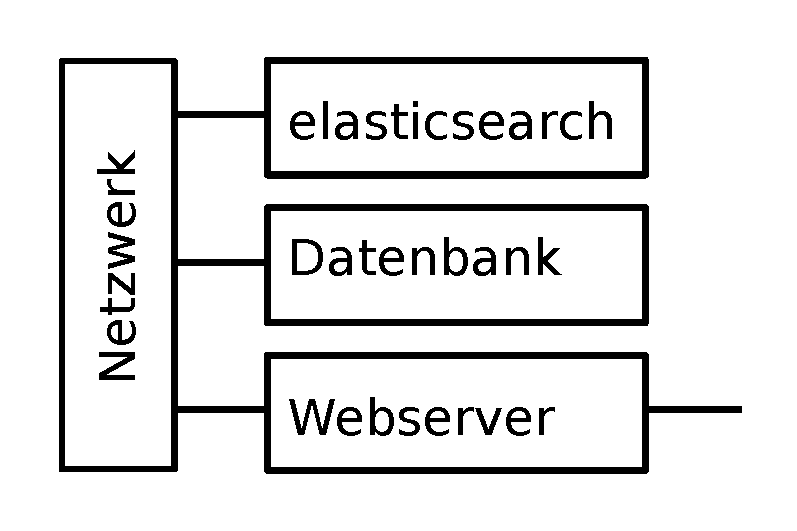
\includegraphics[width=\columnwidth/2]{images/docker-services-example-2.pdf}

  \caption{Beispiel einer Aufteilung in die Services Webserver, Datenbank und
    elasticsearch. Nur der Webserver hat eine externe Netzwerkverbindung.}
  \label{fig:docker-example-simple}
\end{figure}

Eingehende Kommunikation zu Containern wird per Default unterbunden und muss
explizit aktiviert werden. Es ist möglich mehrere Container in ein
gemeinsames Virtuelles Netzwerk zu legen, sodass eine Kommunikation
untereinander stattfinden kann (Reverse-Proxy -> Webseite, Webseite ->
Datenbank) als auch bestimmte Netzwerk Ports des Hosts auf bestimmte Netzwerk
Ports eines Containers zu mappen (Internet -> Reverse-Proxy), siehe Abbildung
\ref{fig:docker-example-extended}.

\begin{figure}
  \includegraphics[width=\columnwidth]{images/docker-services-example.pdf}

  \caption {Erweitertes Beispiel mit zwei getrennten Netzwerken. Loadbalancer
    und Asset   Server haben keinen Zugriff auf die Datenbank, der \texttt{API}
    Server ist auf drei Instanzen skaliert.}
  \label{fig:docker-example-extended}
\end{figure}

\subsubsection{Unterschiede zwischen Docker und VM}

Im Gegensatz zu einer herkömmlichen virtuellen Maschine stellt Docker keine
virtualisierte oder paravirtualisierte Hardware bereit, auf der ein eigenes
Betriebssystem ausgeführt wird. Der Kernel des Hostsystems wird an den Container
weitergereicht und Geräte des Hosts eingebunden was die Performance gegenüber
einer VM verbessert. Dadurch bieten Docker Container allerdings eine größere
Angriffsfläche als eine virtuelle Maschiene. Bei einer VM ist ein Exploit in der
Virtualisierungssoftware nötig, der oft einen Exploit zum erlangen von
Systemrechten innerhalb des virtualisierten Betriebssystem vorraussetzt, um die
VM zu verlassen, gefolgt von einem mit hoher Wahrscheinlichkeit anderem Exploit
um Systemrechte auf dem Hostsystem zu erlangen. Bei Docker Containern reicht
hier ein Kernel Exploit oder ein Exploit im Docker Daemon um Kontrolle über den
Host zu erlangen.

Aufgrund der Deployment Infrastruktur in Form von Image Repositories, sowohl
öffentliche wie Dockerhub als auch private, die selbst betrieben werden können,
ermöglicht Docker sowohl Firmen ihre Services in Images auf privaten
Repositories zu lagern und bei Bedarf auf beliebiger Intrastruktur mit
installierem Docker deployen als auch Open Source Projekten eine lauffähige
konfigurierte Version der Software inklusive aller benötigten Abhängigkeiten 

\subsection{\texttt{RESTFUL API}}

Eine \texttt{RESTFUL API} ist eine, die zustandsfreie \texttt{HTTP} Requests
verwendet zum Zugriff auf Ressourcen via URIs ermöglicht. Ein Request mit
einem der \texttt{HTTP} Verben \texttt{GET}, \texttt{POST}, \texttt{PUT} oder
\texttt{DELETE} gesendet wird greift lesend oder schreibend auf eine Ressource
zu. \texttt{GET} signalisiert die Abfrage von Daten, \texttt{POST} das Verändern
von Daten, \texttt{PUT} das Anlegen neuer Daten und \texttt{DELETE} das Löschen
von Daten. Ein \texttt{GET} Request könnte beispielsweise ein bestimmtes Bild
abrufen, ein anderer eine Datenbank nach allen Einträgen, die einem
mitgeschicktem Filterkriterium entsprechen, durchsuchen. Es ist auch vorstellbar
ein \texttt{RESTFUL API} auf ein definiertes Subset von \texttt{SQL} zu mappen
oder die Steuerung einer Waschmaschiene.

\begin{description}
\item[URI] \mbox{}\\ Ein \texttt{URI} ist ein Uniform Resource Identifier,
  beschrieben in RFC2396\cite{rfc2396}. Es handelt sich dabei um eine Zeichenfolge zur
  Idektifikation von physikalischen oder Abstrakten Ressourcen mit folgender
  Struktur:
\begin{minted}{HTTP}
<Schema>:<schemaspezifischer Anteil>
\end{minted}
Das generische \texttt{URI} Schema entspricht folgender Struktur:
\begin{minted}{HTTP}
<Schema>://<Authorität>/<Pfad>?<Anfrage>

http://blattwerkzeug.de/api/project/blog/image?max_amount=5
\end{minted}
Es sind aber auch andere Strukturen möglich, wie beispielsweise Universial
Resource Name:
\begin{minted}{HTTP}
urn:<Namensraum>:<namensraumspezifische Anteil>

urn:uuid:73ffed65-a912-46dc-8213-83efef4267bf
urn:ietf:rfc:2396
\end{minted}
\item[Ressource] \mbox{}\\ Auf eine Ressource kann zugegriffen werden. Dabei
  kann es sich unter anderem um ein Dokument, ein Bild, den Messwert eines
  Sensors oder einen Datenbankeintrag handeln.
\end{description}

Da die Requests zustandsfrei sind, kann in einem Request nicht auf
einen vorausgegangenen Request zurückgegriffen werden. Zwar werden
duch einen Request eingetretene Datenbankänderungen in der
Datenbankabfrage des nächsten Requests sichtbar, allerdings, existiert
keine Session in der beispielsweise ein Arbeitsverzeichnis festgelegt
oder ein von allen Folgerequests verwendeter Namensraum ausgewählt
werden kann. Jeder Request muss alle zu seiner Verarbeitung
notwendigen Informationen selbst beinhalten.

\subsection{\texttt{Model-View-Controller}}
Model View Controller ist ein zum bearbeiten von Inhaltsanfragen geeignetes
Konzept. Daten werden nach durch ein Model beschrieben und strukturiert und
verwaltet, ihre Darstellung durch den View festgelegt und die Webrequests vom
Controller behandelt. So werden Datenhaltung, Darstellung und Buisiness Logic
von einander getrennt und können bis zu einem gewissen Grad unabhängig von
einander überarbeitet werden. Abbildung \ref{fig:mvc} zeigt die Interaktion
zwischen Model, View und Controller.

\begin{figure}
  \centering
  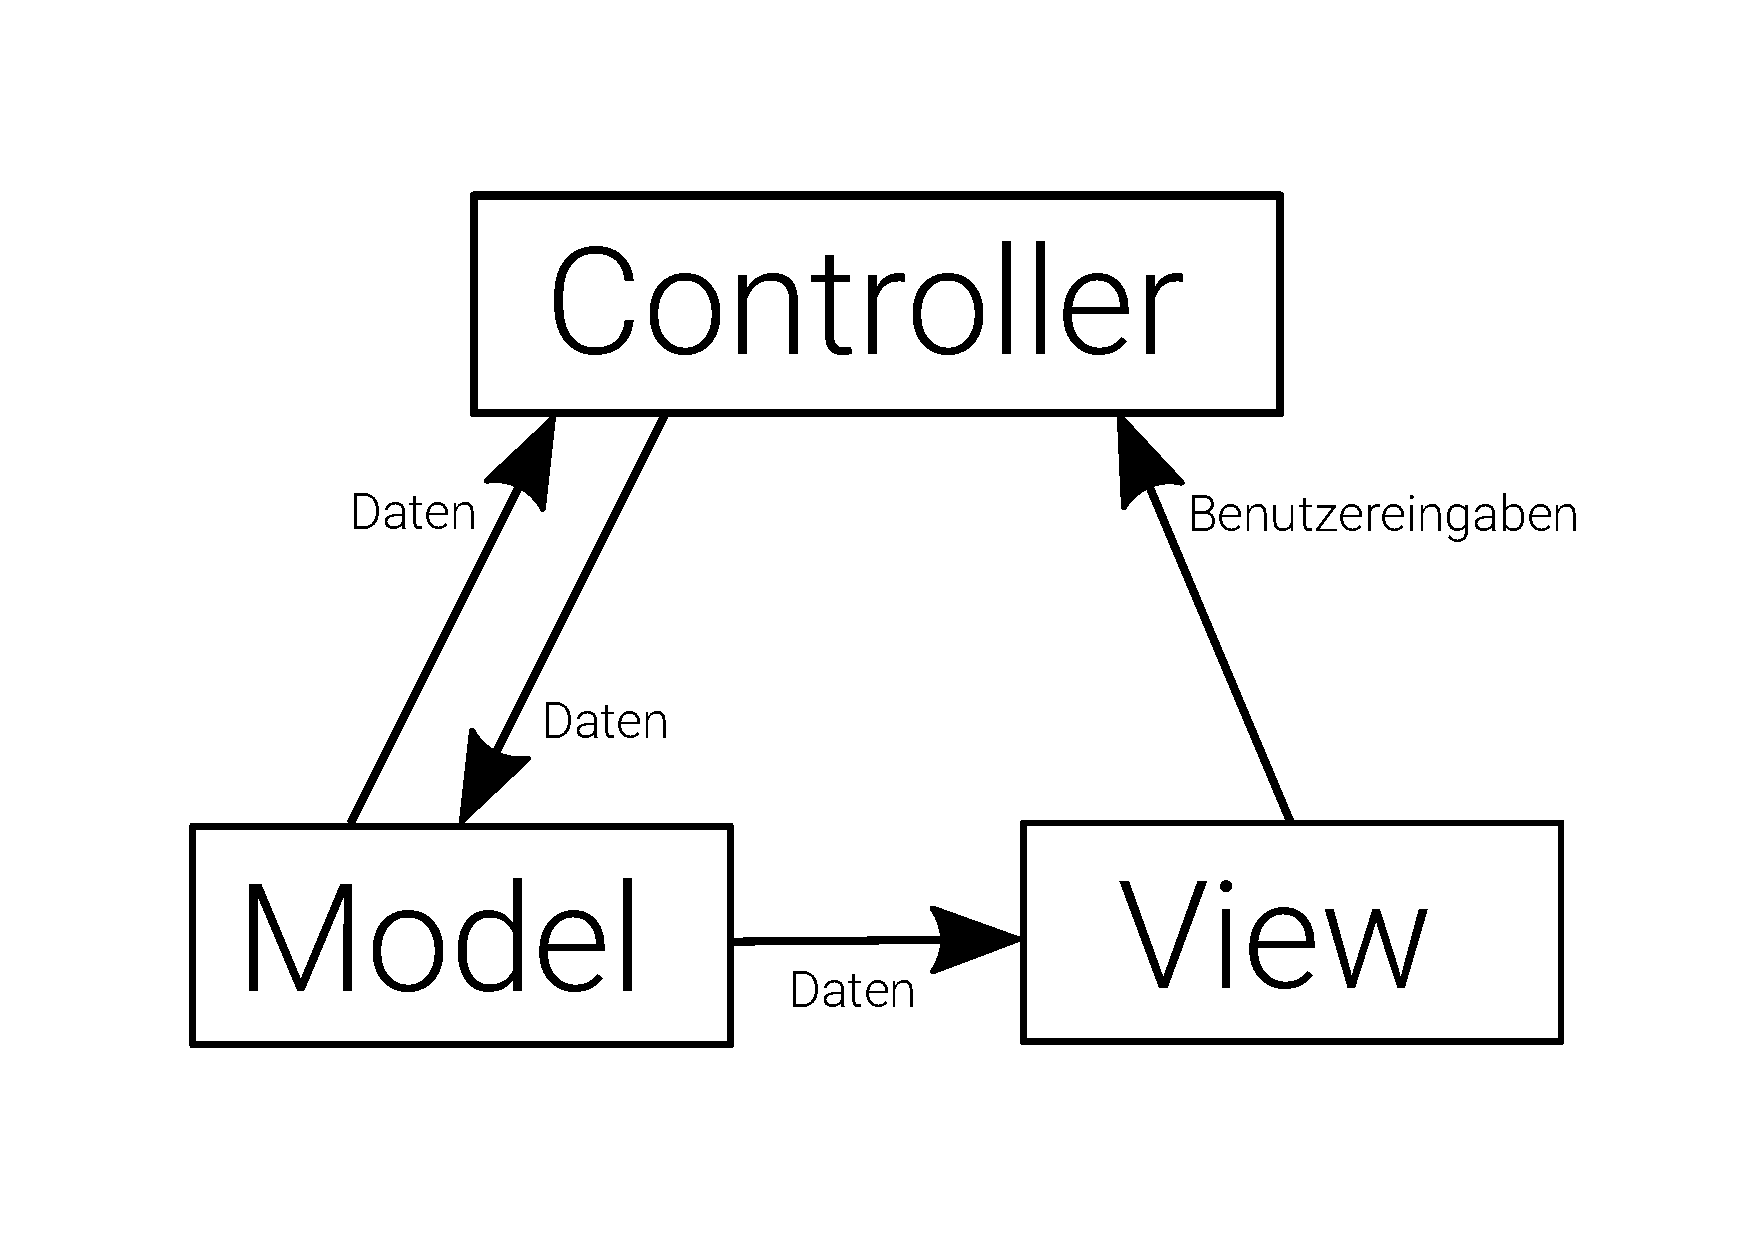
\includegraphics[width=\columnwidth]{images/mvc.pdf}
  \caption{MVC Übersicht}
  \label{fig:mvc}
\end{figure}

\subsection{Kurze Beschreibung von Angular}

Angular ist eine App Platform für Webbrowser und macht vom MVC Modell gebrauch.
Es gibt Components, Templates und Interfaces.
\begin{description}
  \item[Template] \mbox{} \\ Templates beinhalten \texttt{HTML} und Angular
    Bindings, die Daten aus dem Model einfügen und Events an Funktionen binden.
  \item[Interface] \mbox{} \\ Auch wenn Interfaces nicht direkt die Rolle des
    Models einnehmen, sind sie die Clientseitige Repräsenation des Models, das
    Serverseitig, meist in einer Datenbank abgelegt ist.
  \item[Component] \mbox{} \\ Komponenten nehmen in Angular die Rolle des
    Controllers ein und stellt Funktionen bereit, die auf Ereignisse reagieren
    und mit dem Model interagieren.
\end{description}

\subsection{Lizenzen}

Wer ein Bild, Text oder anderes Werk mit Schöpfungshöhe erstellt hat in
Deutschland als Urheber alle Rechte an besagtem Werk. Um jemand anderem die
Nutzung des Werkes zu ermöglichen muss der Urheber dem Nutzer eine
Nutzungslizenz erteilen, die definiert in welcher Art und Weise der Nutzer das
Werk nutzen darf und welche Bedingungen er dabei erfüllen muss, in anderen
Jurisdiktion gelten ähnliche aber im Detail andere Regeln hierfür.

Der Inhalt der Lizenz ist beliebig, unterliegt je nach Jurisdiktion allerdings
gewissen Einschränkungen. Desweiteren ist die Bedeutung des Wortlauts
Interpretationssache des Richters, sollte es zu einem Rechtsstreit kommen,
weshalb Unkundigen davon abgeraten wird eigene Lizenztexte zu verfassen und ohne
Rücksprache mit einem Fachkundigen zu verwenden, da sich die juristische Sprache
von der Alltagssprache unterscheidet und ein einziges Wort, dass Aufgrund der
Wohlklingenden Satzmelodie eingefügt wurde einen Kompletten Paragraphen
wirkungslos machen kann.

Um das Teilen eigener Werke mit anderen rechtssicher zu ermöglichen, ohne in
eine juristische Falle zu tappen wurden von der zu diesem Zweck in den USA
gegründeten Organisation Creative Commons die Creative Commons Lizenzen
entworfen. Anfangs befassten sich diese Lizenzen nur mit US-amerikanischem
Recht, und stellten sich außerdem als Überarbeitungsbedürftig heraus. Die
aktuellen Fassungen in der Version 4.0 sind allerdings Internationalisiert mit
offiziellen Übersetzungen, die auf die jeweiligen Besonderheiten der jeweiligen
Jurisdiktionen eingehen. \cite{CC}

Die regulären Creative Commons Lizenzen sind

\begin{tabular}{ c l l }
  & \texttt{CC BY \cite{CC-BY}} & Attribution \\
  & \texttt{CC BY-SA \cite{CC-BY-SA}} & Attribution + ShareAlike \\
  & \texttt{CC BY-ND \cite{CC-BY-ND}} & Attribution + NoDerivatives \\
  & \texttt{CC BY-NC \cite{CC-BY-NC}} & Attribution + Noncommercial \\
  & \texttt{CC BY-NC-SA \cite{CC-BY-NC-SA}} & Attribution + Noncommercial + ShareAlike \\
  & \texttt{CC BY-NC-ND \cite{CC-BY-NC-ND}} &  Attribution + Noncommercial + NoDerivatives
\end{tabular}

wobei die Begriffe folgende Bedeutung haben:
\begin{description}
  \item[Attribution (\texttt{BY})] \mbox{} \\ Nutzer muss Lizenz und Urheber
    derklarieren.
  \item[ShareAlike (\texttt{SA})] \mbox{} \\ Abgeleitete Werke müssen unter
    selber Lizenz veröffentlicht werden.
  \item[NoDerivatives] \mbox{} \\ Es dürfen keine abgeleiteten Werke
    veröffentlicht werden.
  \item[Noncommercial] \mbox{} \\ Kommerzielle Nutzung ist untersagt.
\end{description}

Da die Begriffe Gemeinfrei oder Public Domain keine Weltweit gültige
übereinstimmende Definition haben, wurde zusätzlich die Creative Commons Zero
Lizenz (\texttt{CC0}) geschaffen, um Werke jedem, zu jedem Zweck und ohne Einschränkungen
zur Verfügung zu stellen.

%%% Local Variables:
%%% mode: latex
%%% TeX-master: "thesis"
%%% End:
